
    \subsection*{Modifying our sigmoid}
    
        What happens when you modify the \textbf{parameters} of an LLC? Let's find out.
        
        We'll use a 1-D input: our variables will be $\theta$ (scalar) and $\theta_0$: $\theta x + \theta_0$
        
        \begin{figure}[H]
            \centering
            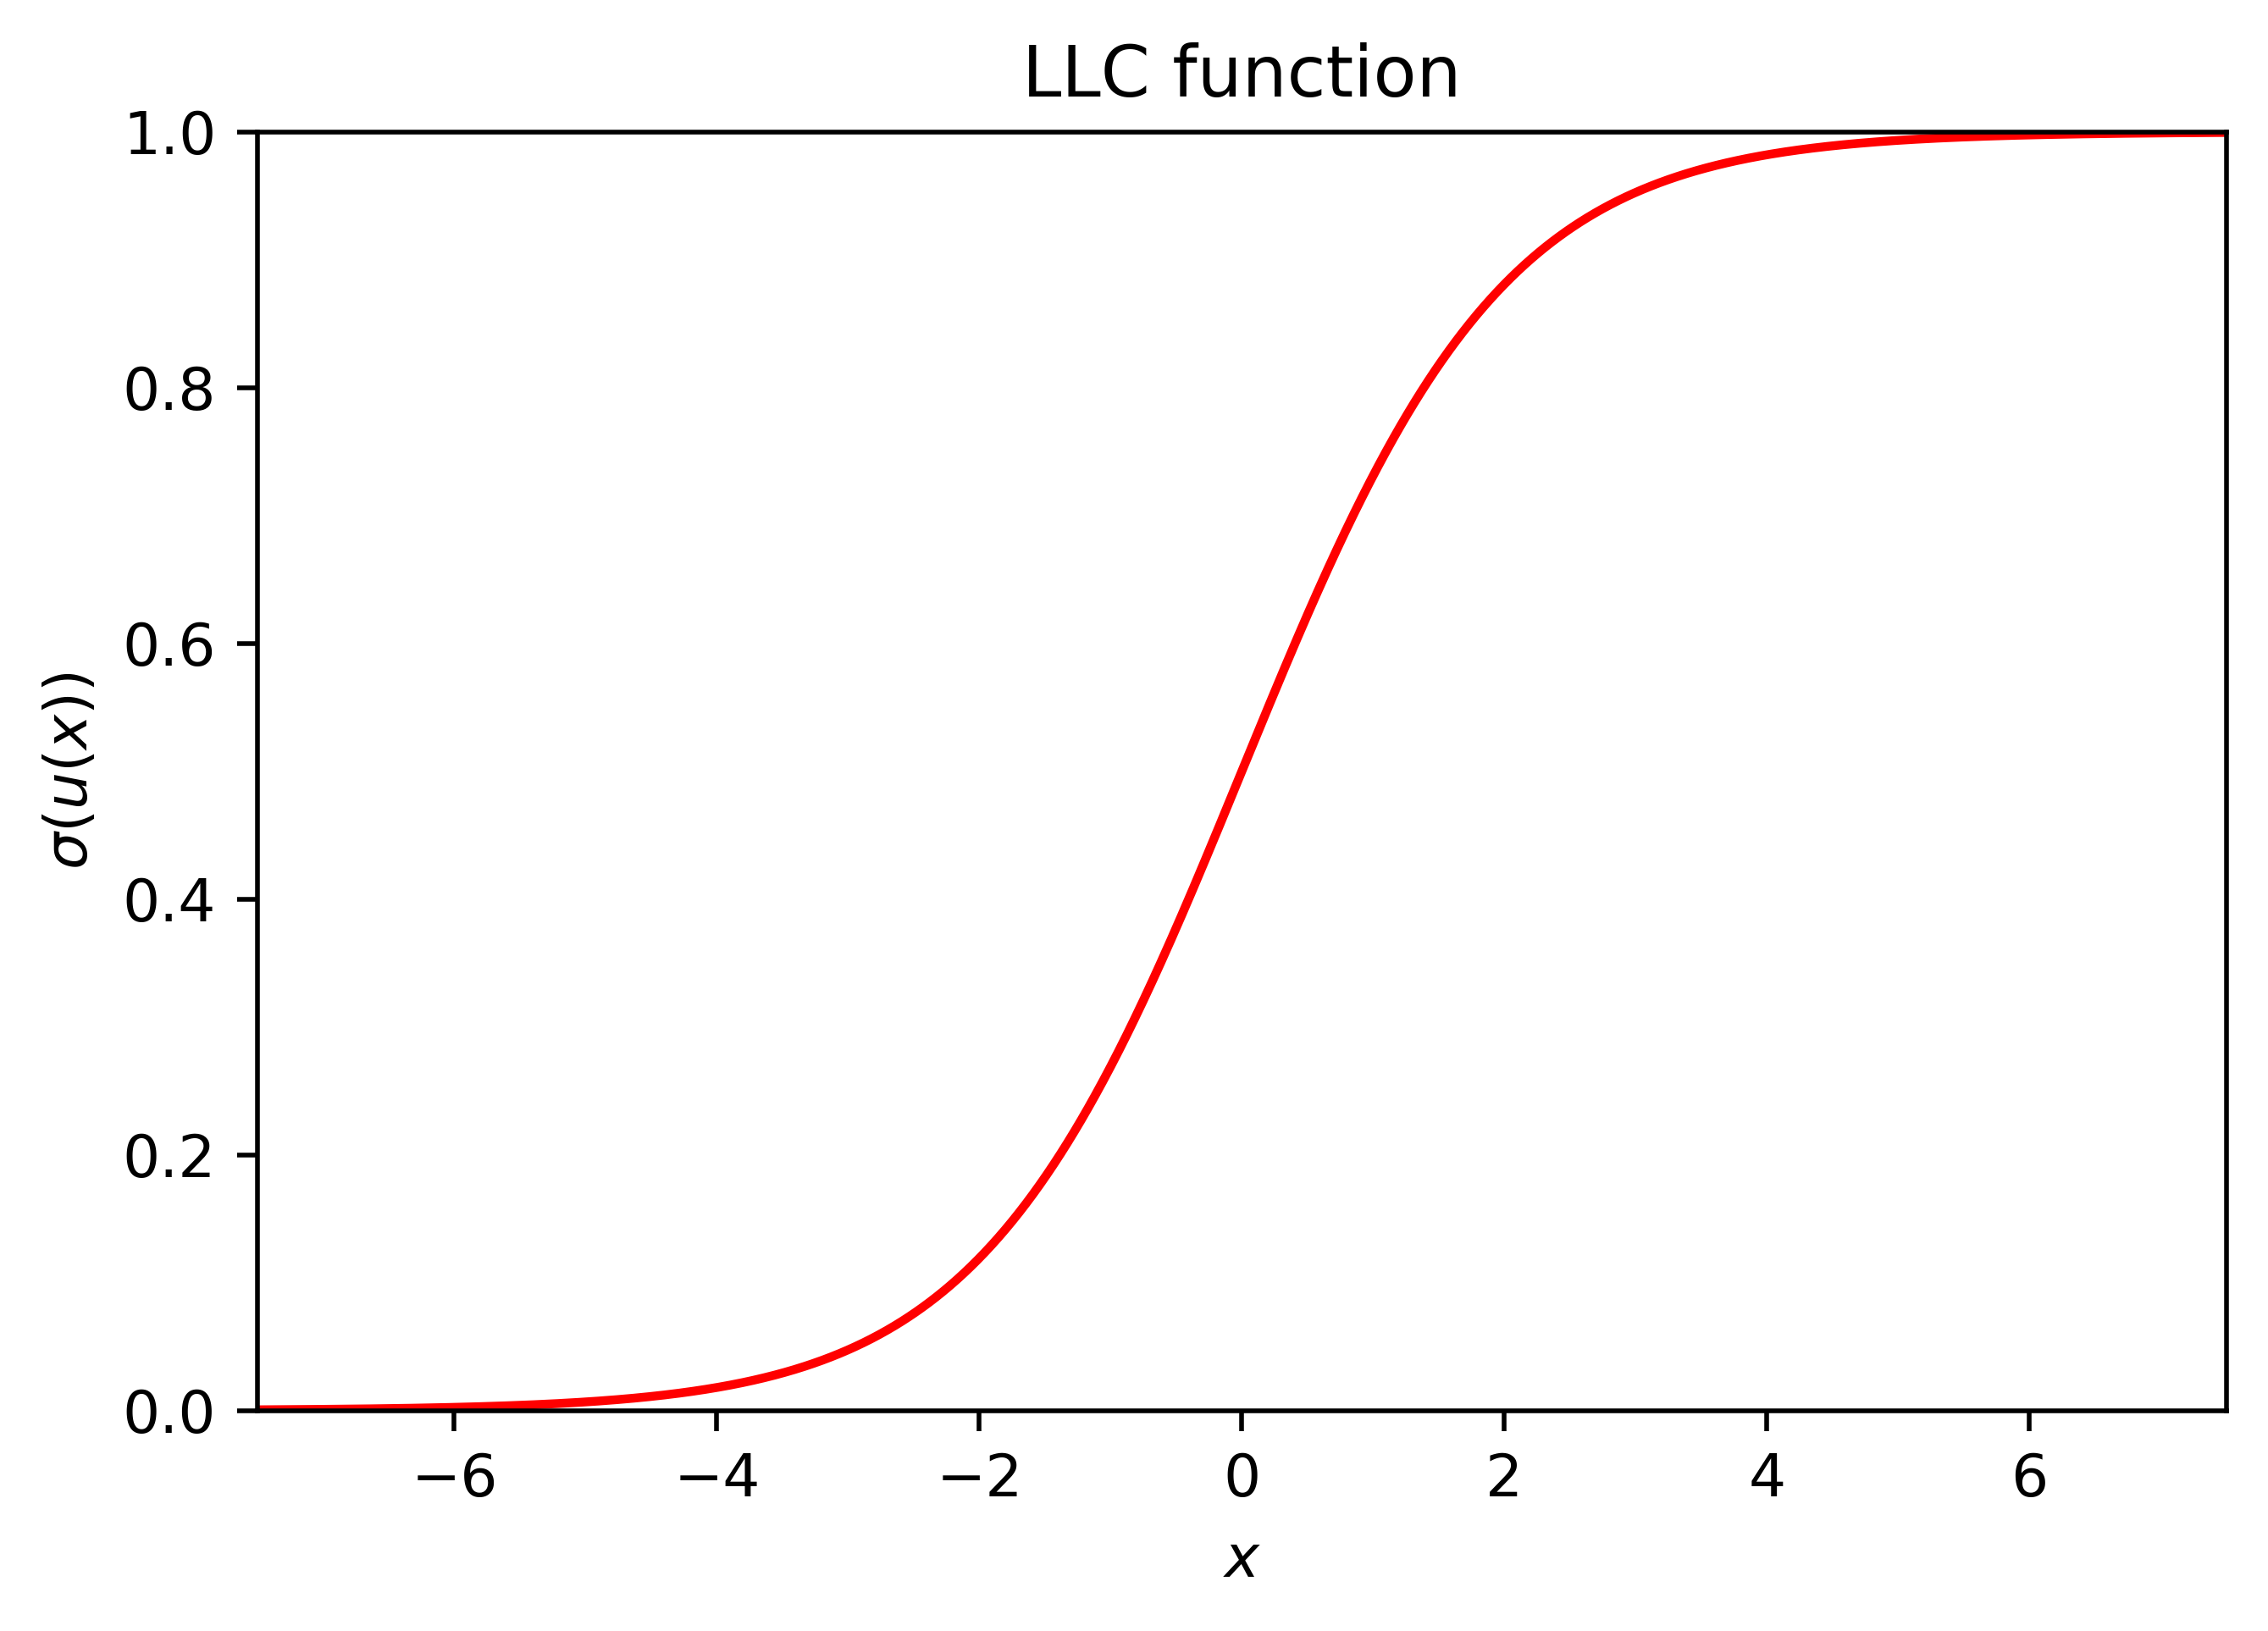
\includegraphics[width=70mm,scale=0.5]{images/classification_images/llc_func.png}
            \caption*{Our baseline LLC: $u(x)=1x+0 $}
        \end{figure}
        
        What if we shift by increasing $\theta_0$?
        
        \begin{figure}[H]
            \centering
            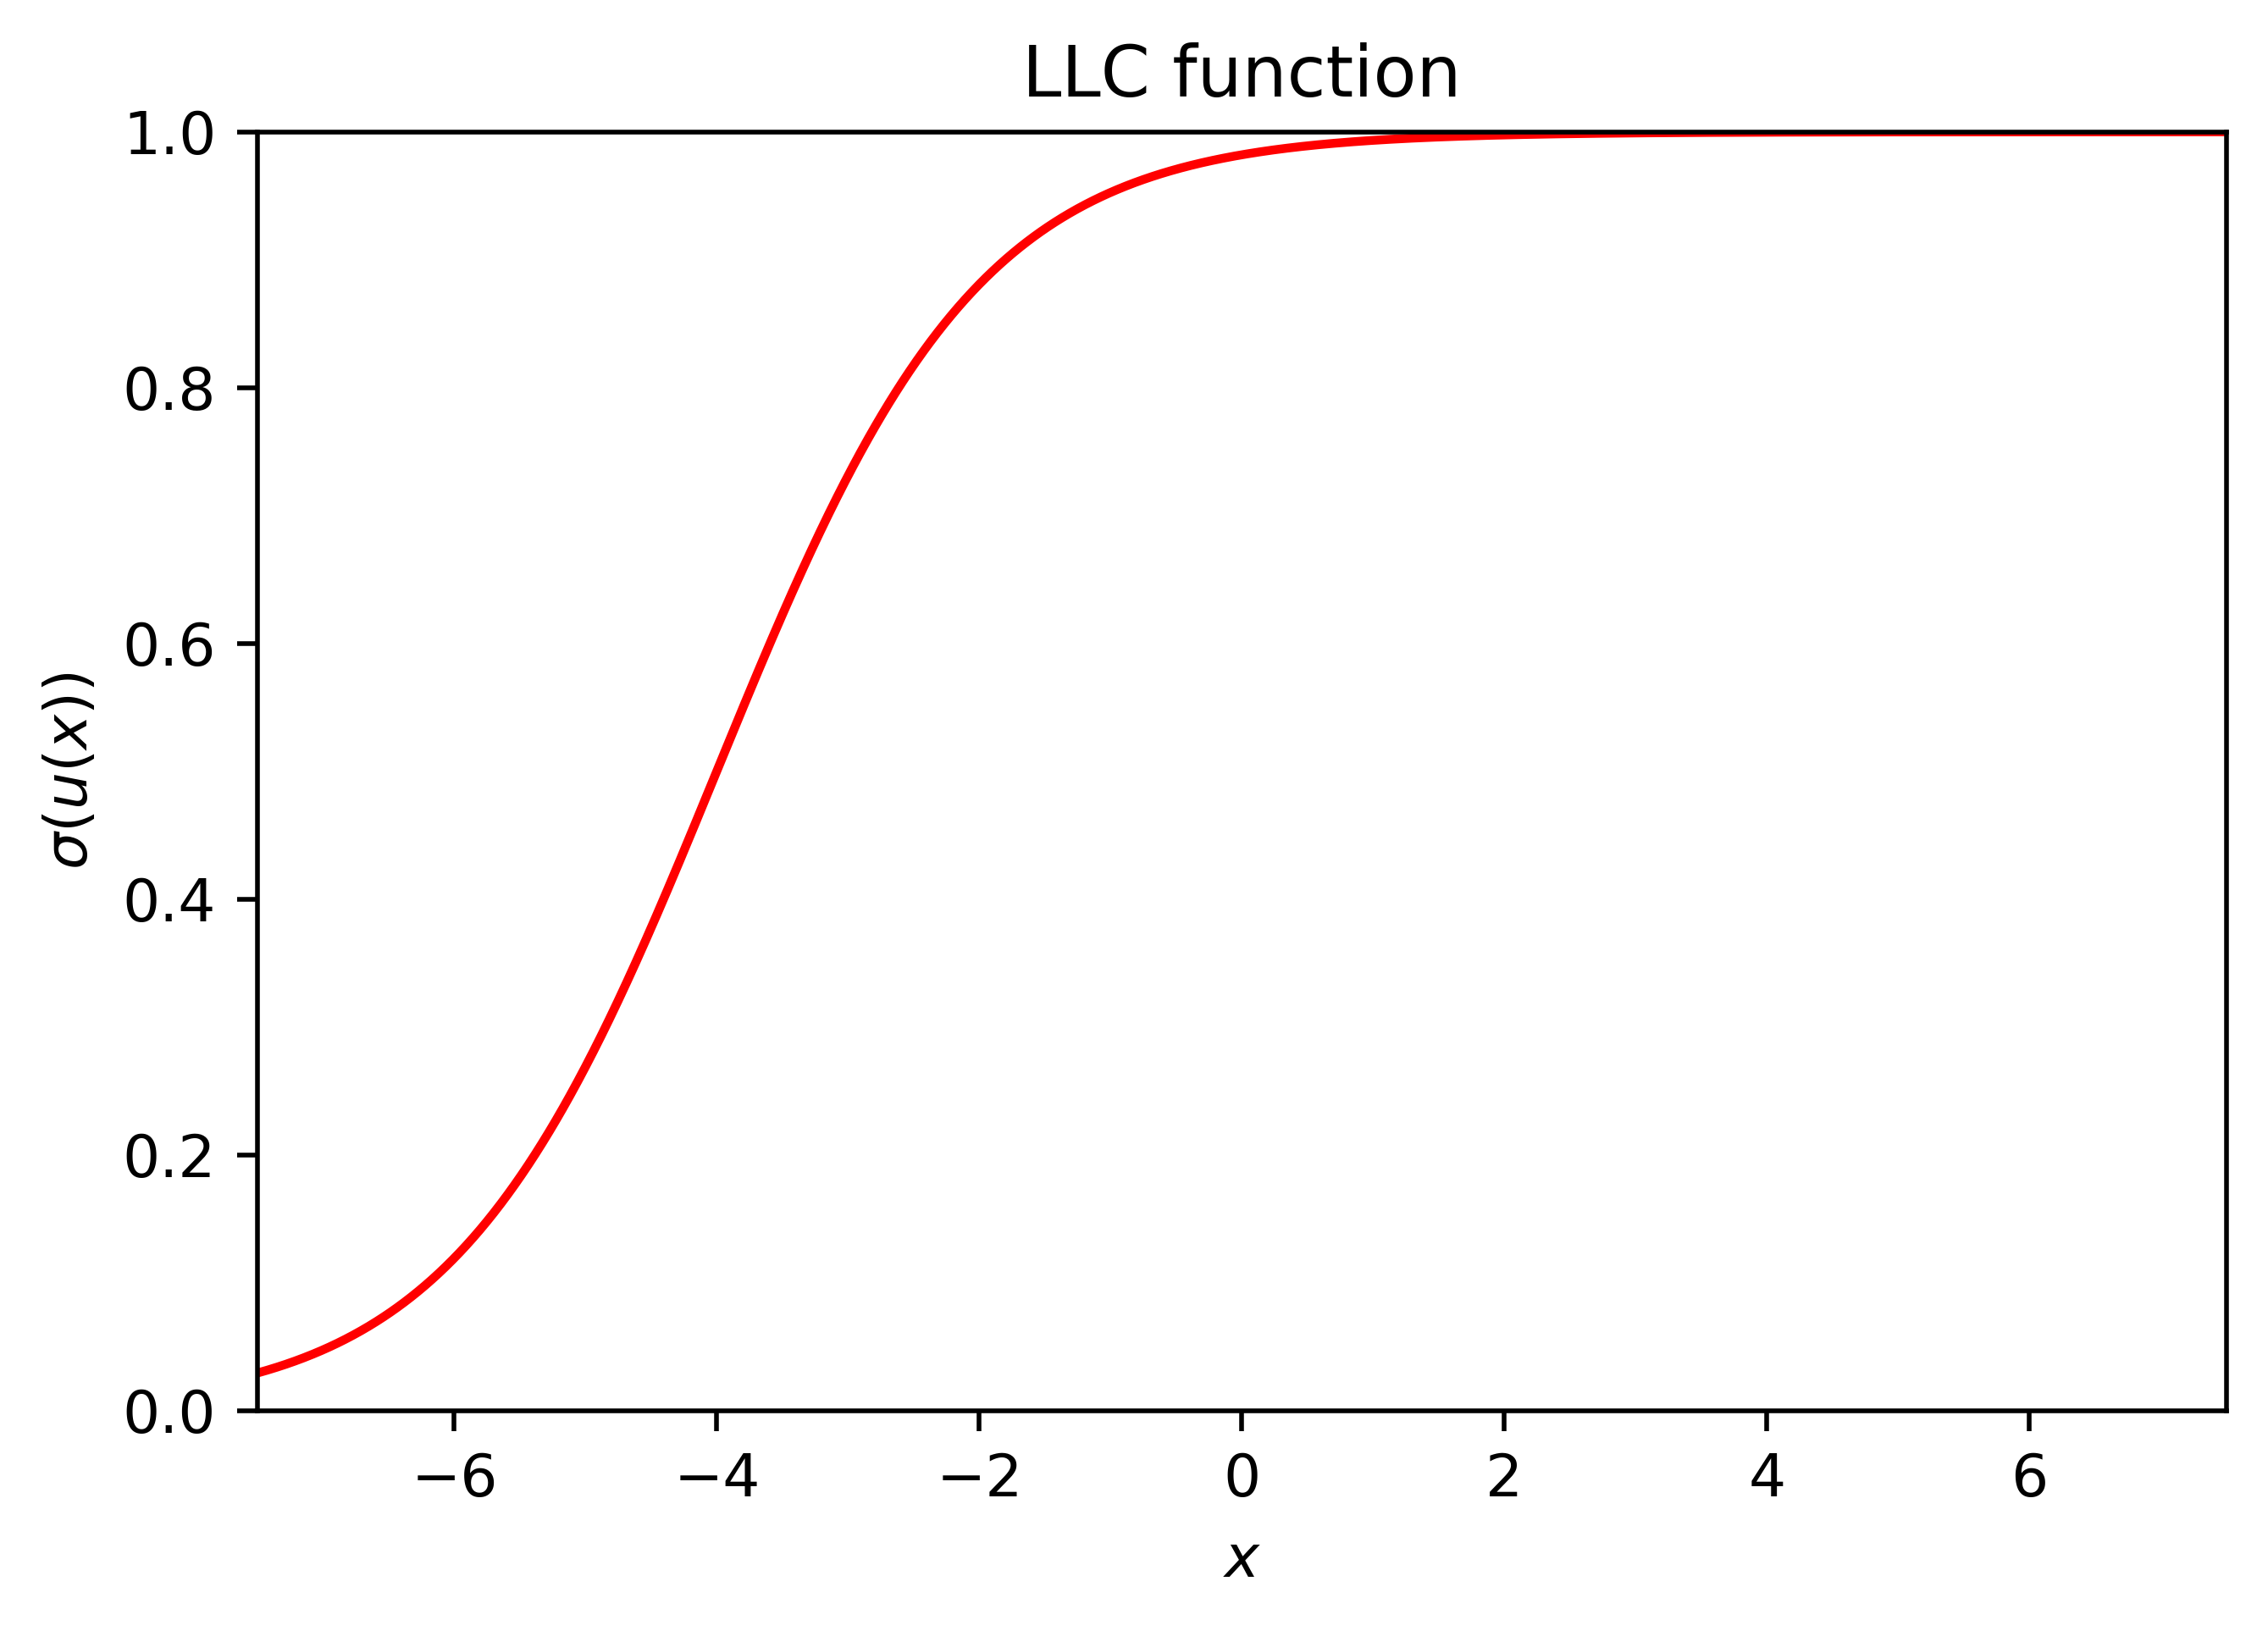
\includegraphics[width=70mm,scale=0.5]{images/classification_images/theta_0_+2.png}
            \caption*{Our shifted LLC: $u(x)=1x+4 $. $\theta_0$ shifts us along the $x$-axis!}
        \end{figure}
        
         Just like before, it \textbf{shifts} us in the \textbf{opposite} direction: if $\theta_0$ is \textbf{positive}, we shift in the \textbf{negative} direction, and vice versa.
         
         What if we increase the magnitude of $\theta$!
         
         \begin{figure}[H]
            \centering
            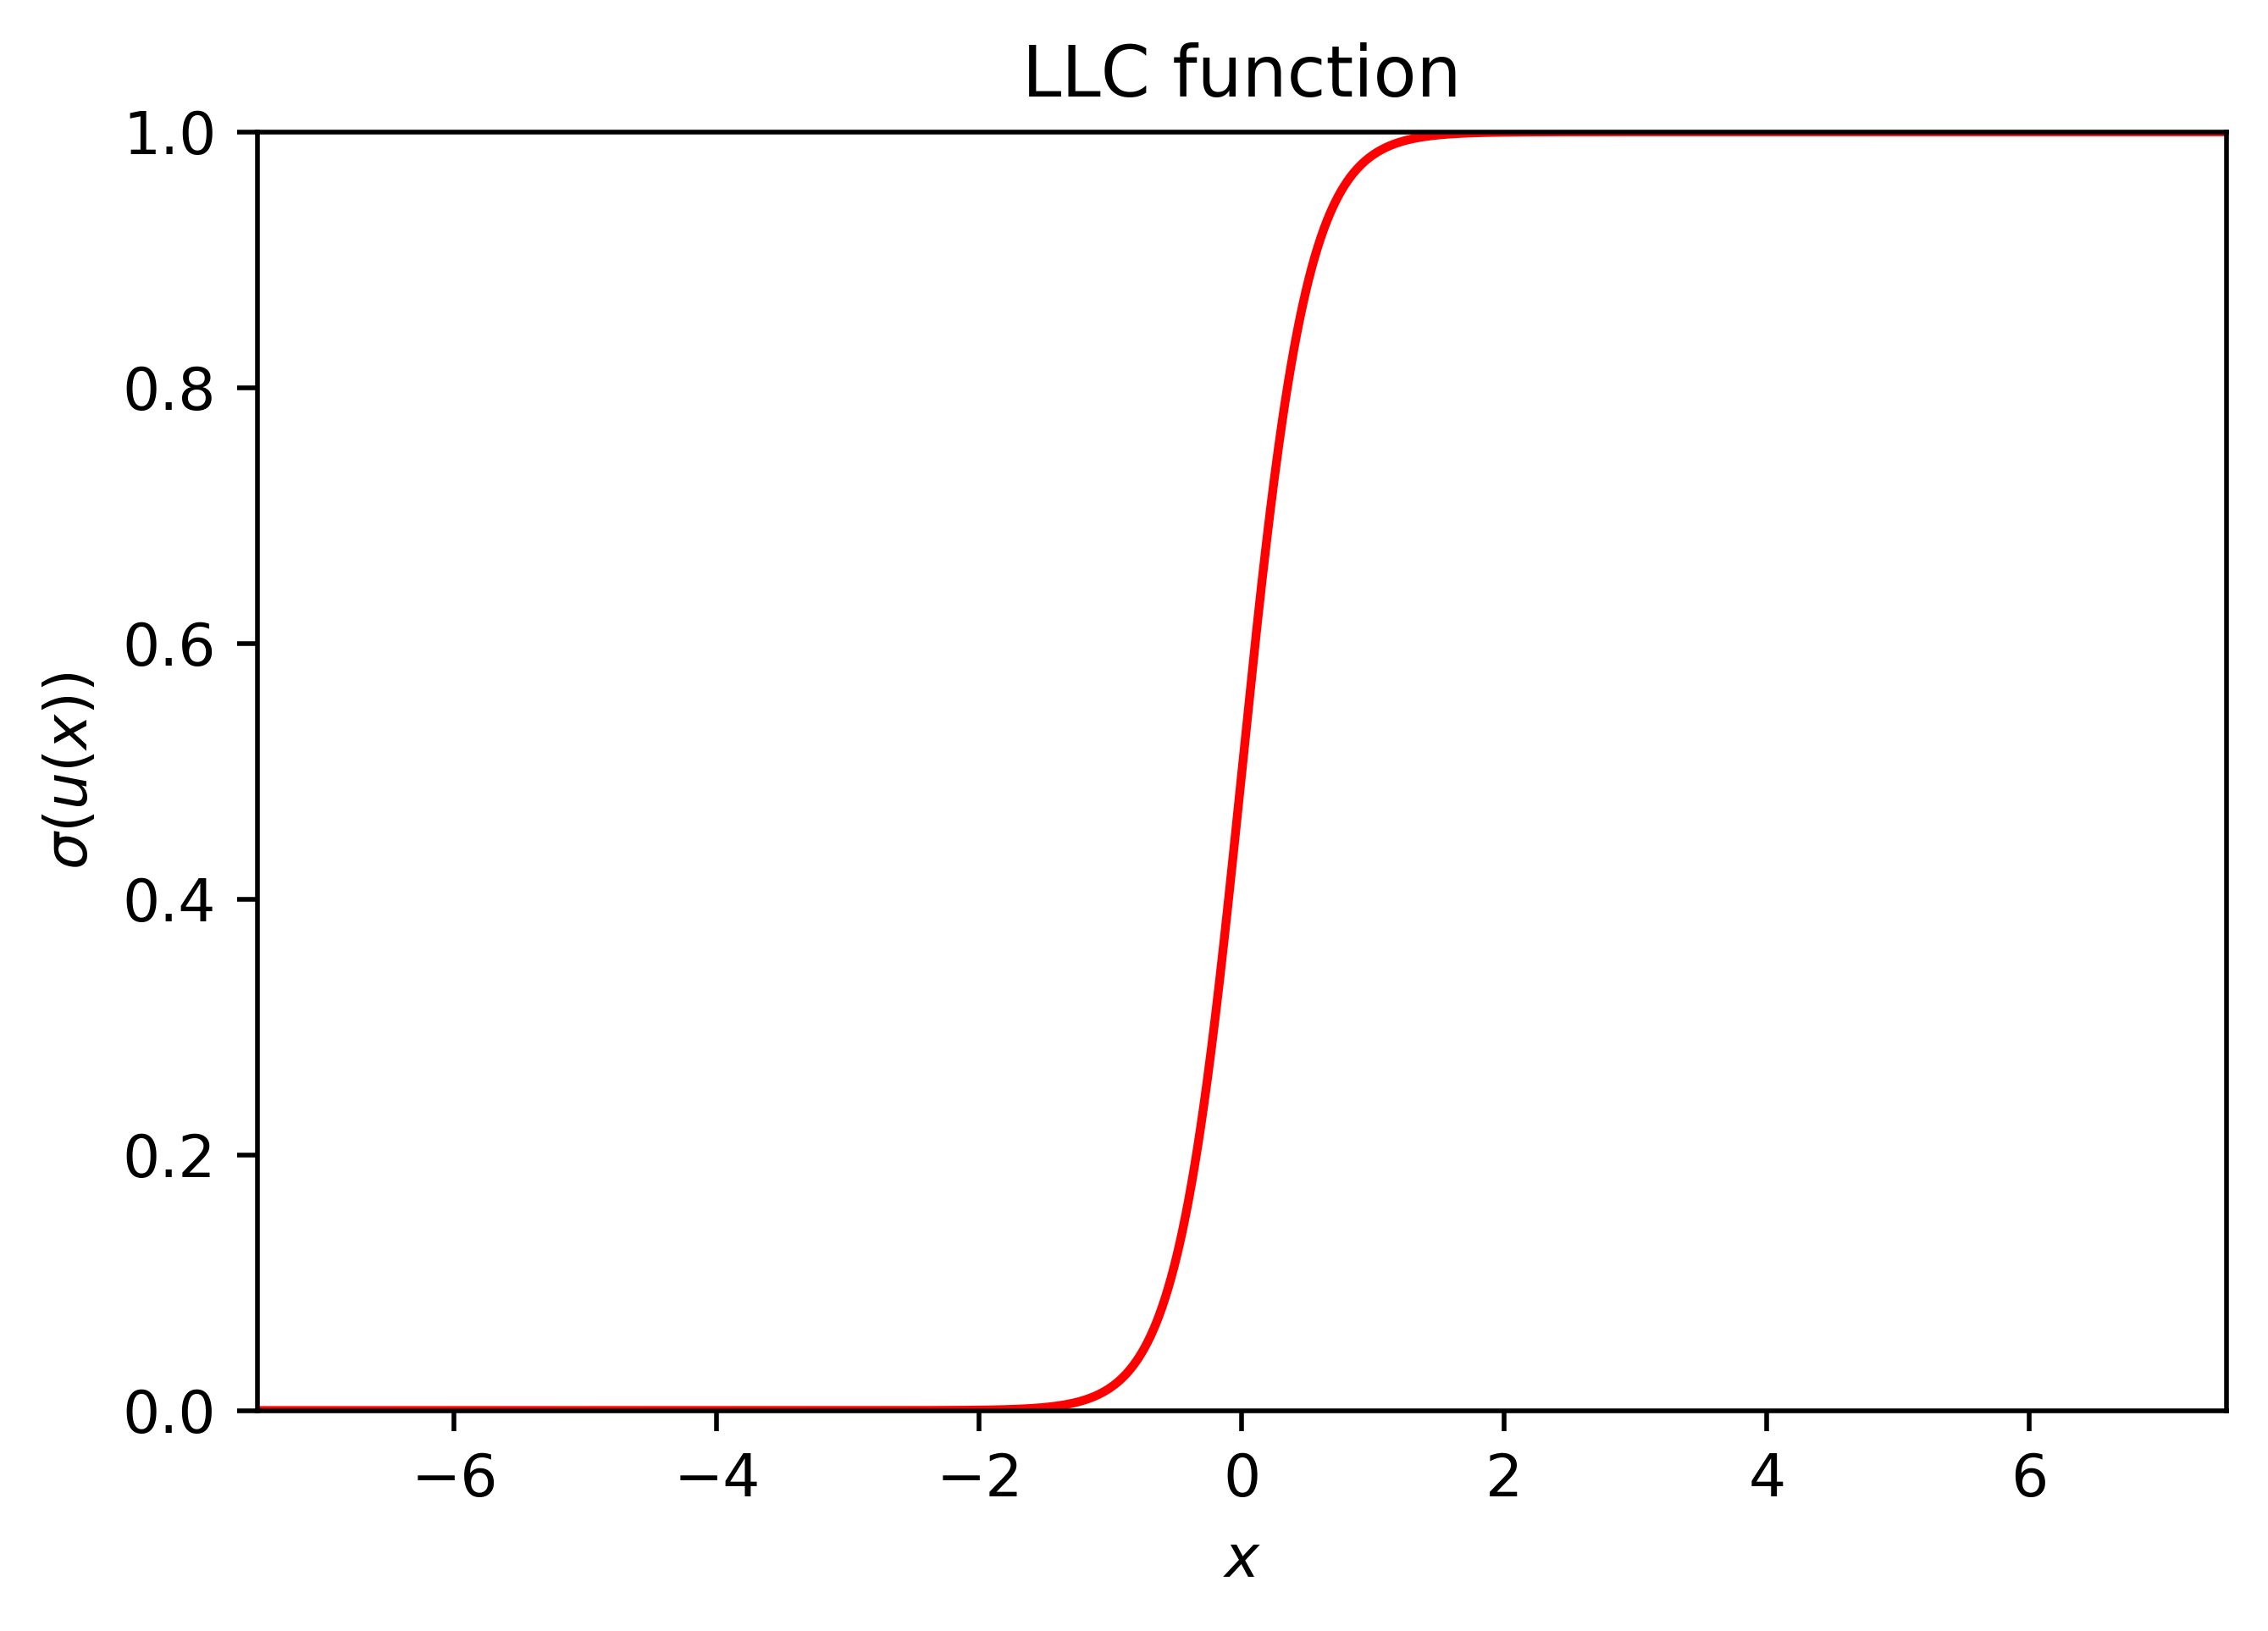
\includegraphics[width=70mm,scale=0.5]{images/classification_images/theta_x4.png}
            \caption*{Our new LLC: $u(x)=4x$. Increasing $\theta$ makes our function steeper!}
        \end{figure}
        
        Making the magnitude of $\theta$ larger makes our function \textbf{change} faster. 
        
        This makes some sense: if $\theta$ (linear slope of $u(x)$) makes $u(x)$ \textbf{change} faster, it will make $\sigma(u)$ change faster \textbf{too}.
        
        You can combine these changes as well: you can shift your LLC with $\theta_0$, and also make it steeper/less steep by changing magnitude of $\theta$.\\
        
        \begin{concept}
            When working with \vocab{sigmoids}, you can \purp{transform} them using your \gren{parameters}:\\
            
            \begin{itemize}
                \item A higher \purp{magnitude} $\norm{\theta}$ makes the slope \gren{steeper}, and answers more \gren{confident}.
                
                \item \purp{Increasing} $\theta_0$ \gren{shifts} the sigmoid in the $-\theta$ \gren{direction}, and vice versa.
            \end{itemize}
        \end{concept}
        
    \subsection*{Viewing our sigmoid in 3D}
        
        Let's quickly take a look at a sigmoid in 3D, with two inputs:
        
        \begin{figure}[H]
            \centering
            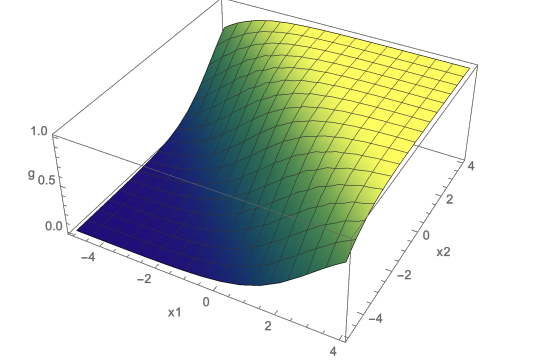
\includegraphics[width=70mm,scale=0.5]{images/classification_images/llc_3d.png}
        \end{figure}
        
        As you can see, you get mostly the same shape: if you look at it from the side, it's exactly the same, in fact! Just stretched out into 3D.
        

    \subsection*{LLCs and LCs have the same boundary}
        
        One more important thing to note: noticed that we set $\sigma_{thresh}=.5$, because that was when $u(x)=0$.
        
        This means that, if our threshold is $0.5$, then the boundary of our LLC should look exactly the same as if it were LC: the only difference is the values that we \textit{can't} see:
        
        \begin{figure}[H]
            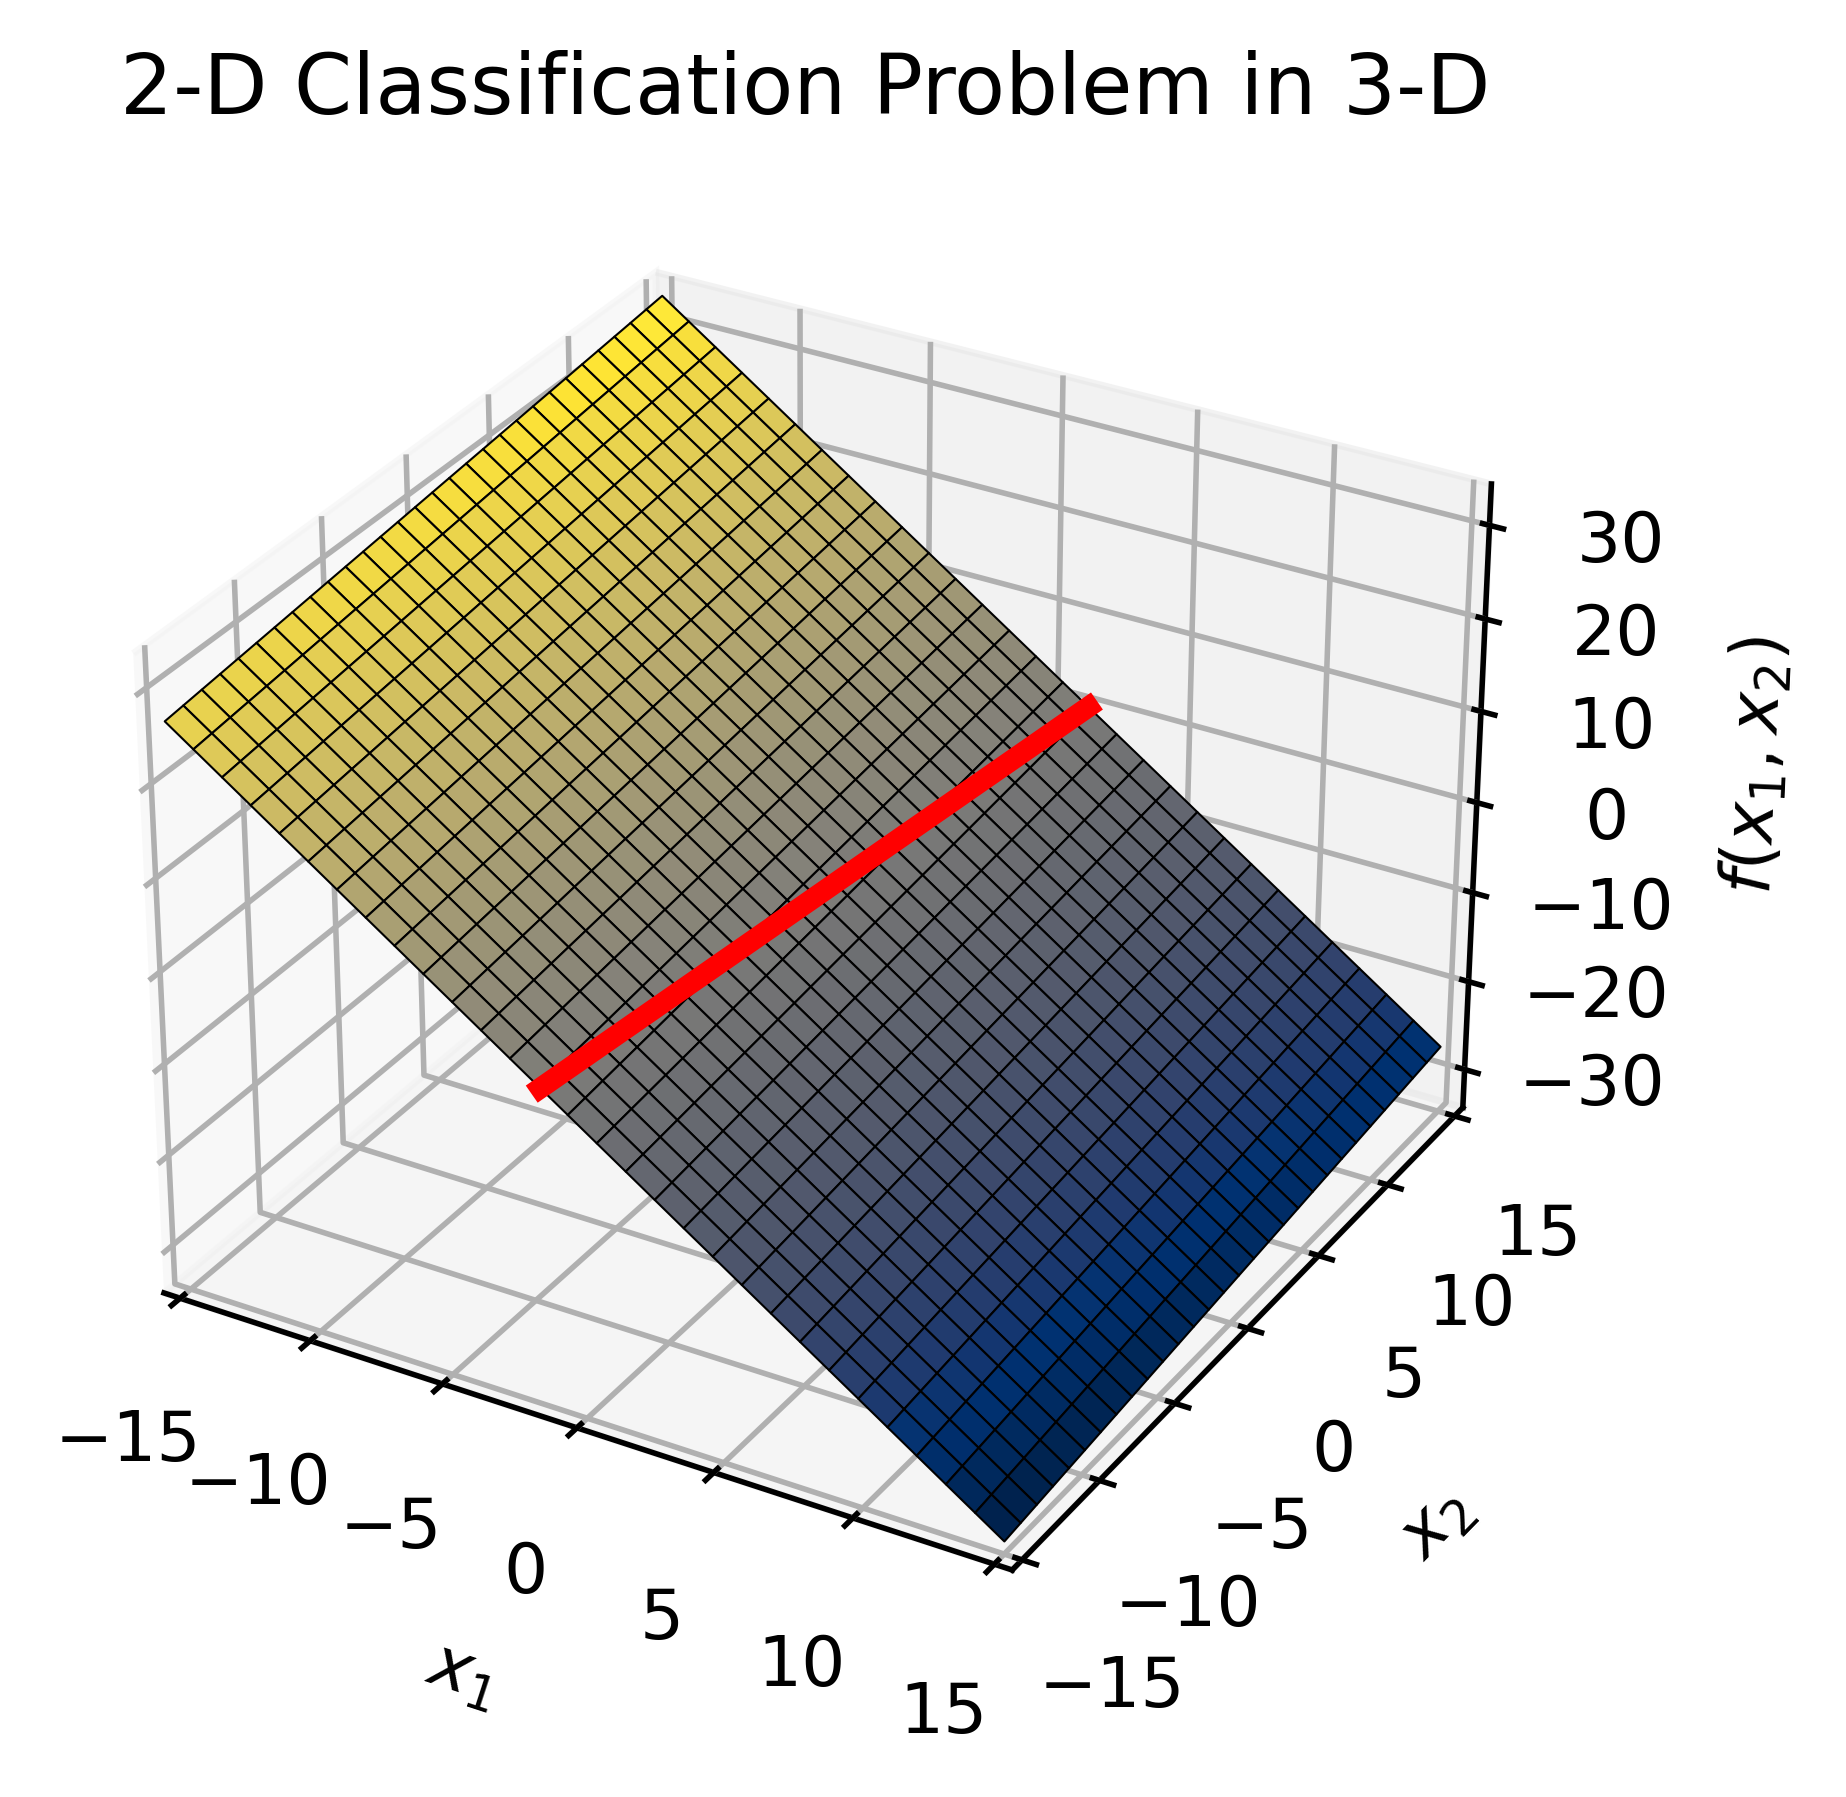
\includegraphics[width=70mm,scale=0.5]{images/classification_images/2d_classification_in_3d_plane.png}
            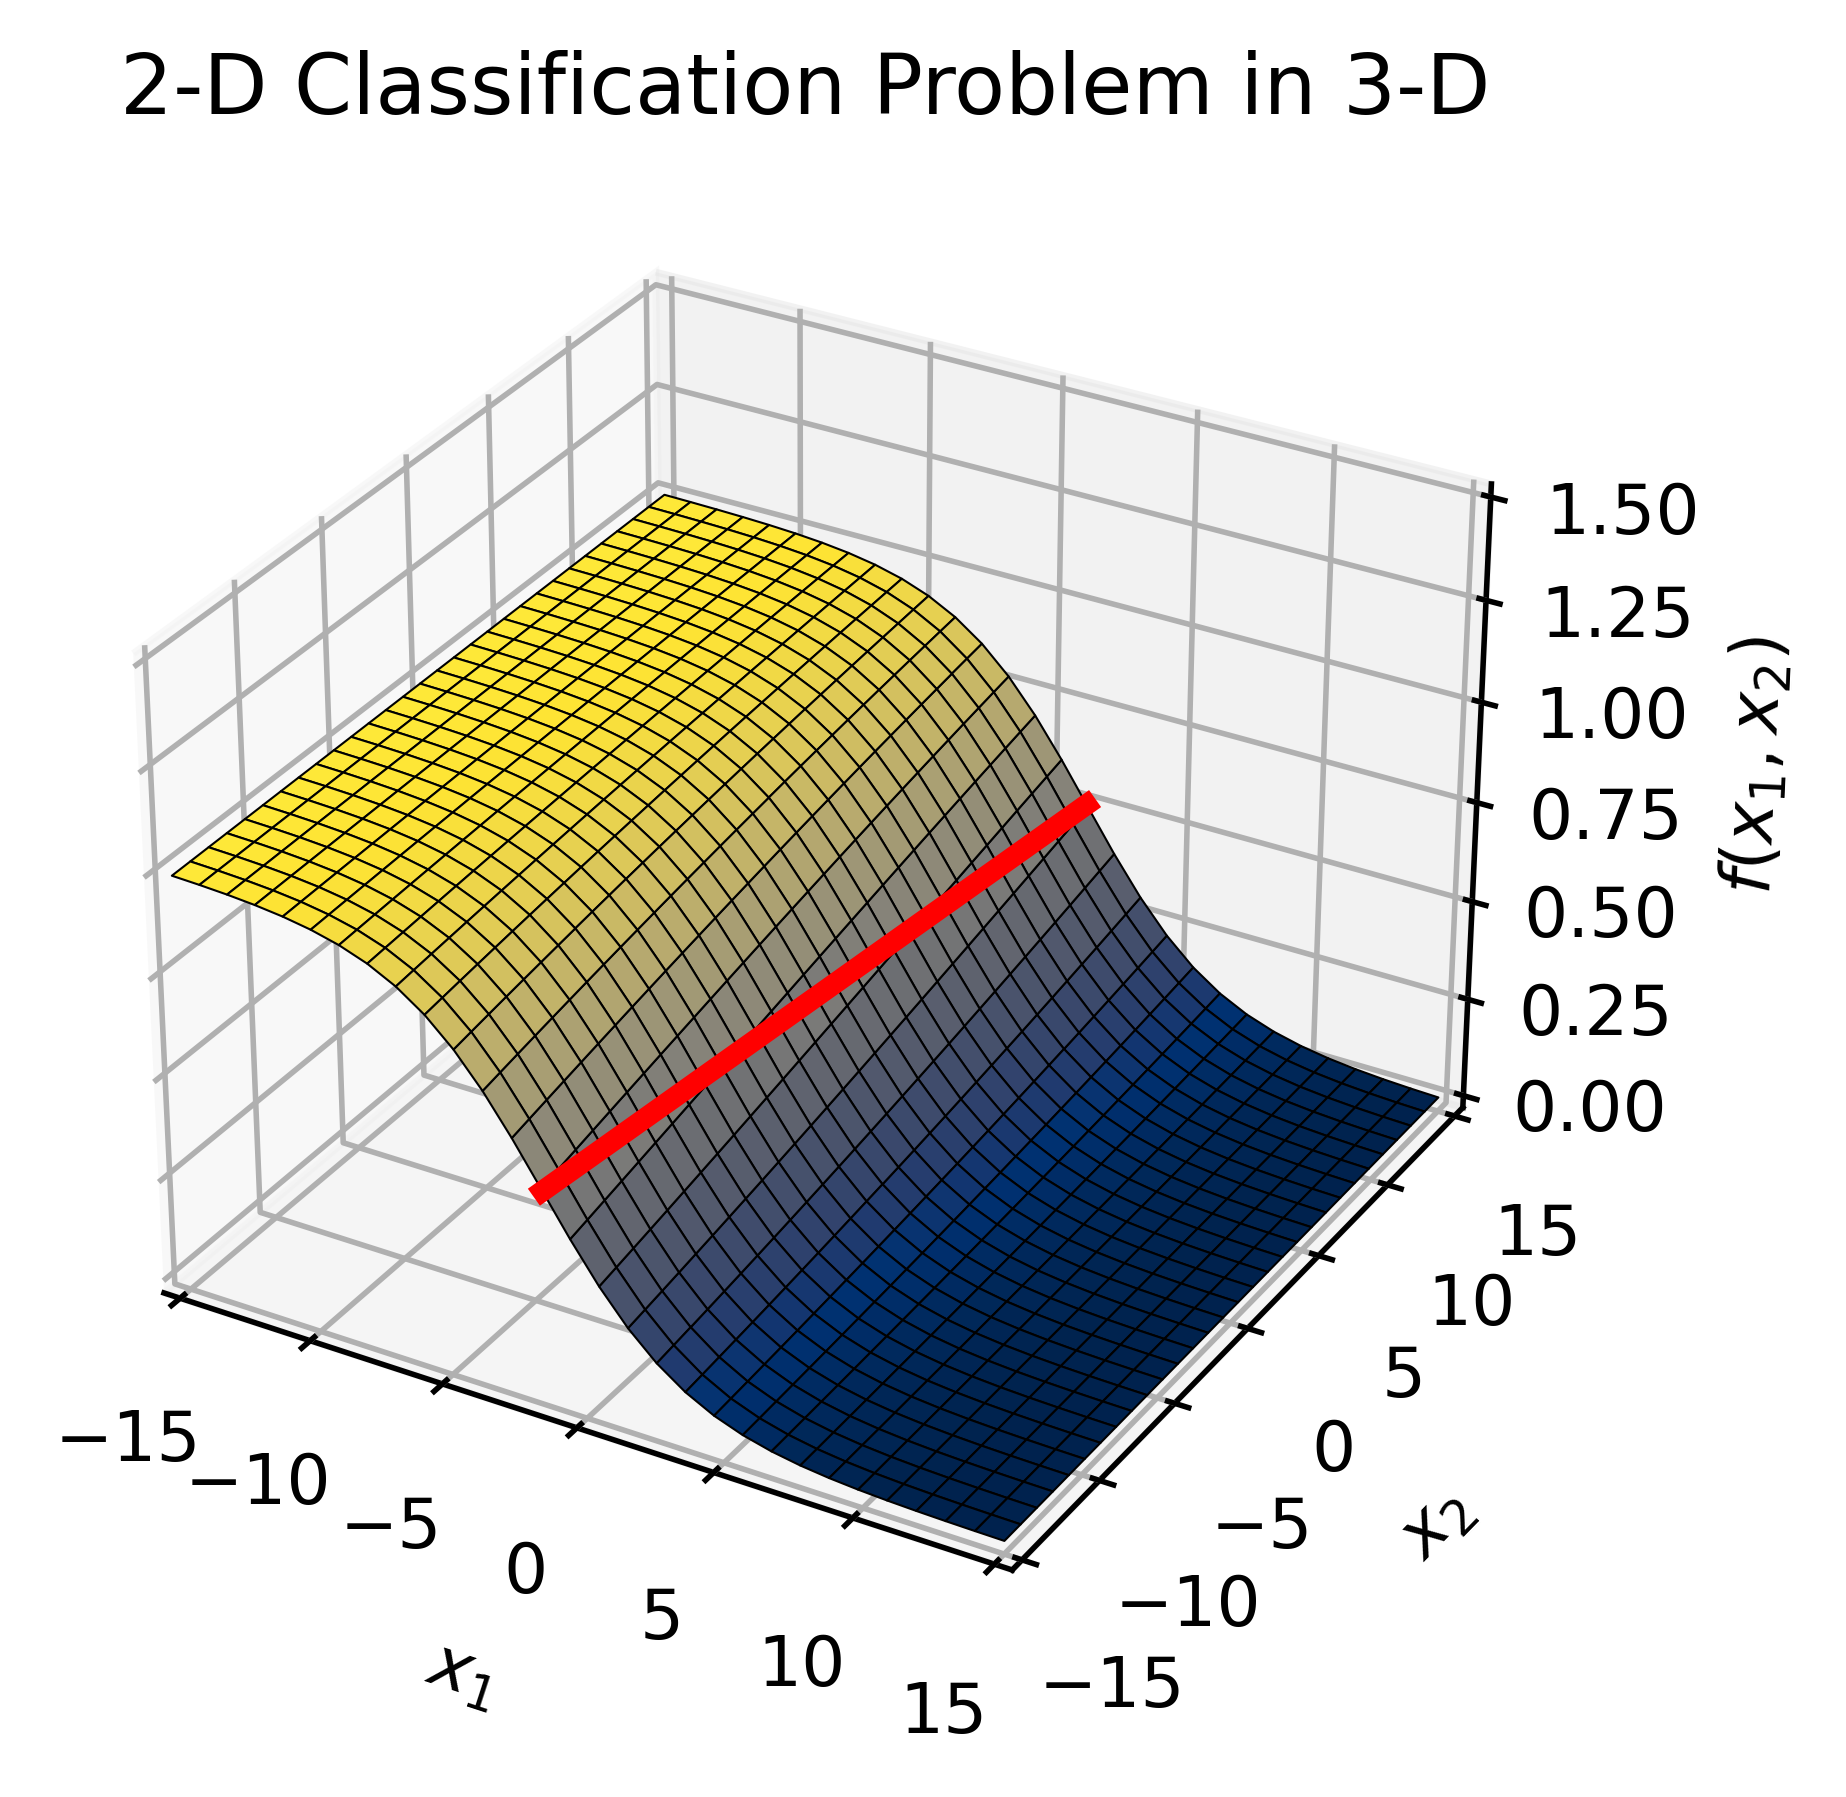
\includegraphics[width=70mm,scale=0.5]{images/classification_images/2d_classification_in_3d_sigmoid.png}
            
            \caption*{Despite having different shapes in 3D, they both create 2-D \textbf{linear} classifiers: on the left, $u(x)=0$, and on the right, $\sigma(u)=.5$.}
        \end{figure}
        
        One way to think about this difference is that while one may be logistic, they are both \textbf{linear}: they both create the same \textbf{linear separator}.
        
        The main benefit of switching to LLC is that $\sigma(u)$ has a useful \textbf{gradient}, while sign$(u)$ does \textbf{not}, so we can do \textbf{gradient descent}.
            \note{The probabilistic interpretation is also more appropriate: we shouldn't be fully confident in our answers.}
            
        Even if we adjust our threshold $\sigma_{thresh}$, that will simply shift the linear classifier.\\
        
        \begin{concept}
            \vocab{LLCs} (Linear Logistic Classifiers) and \vocab{LCs} (Linear Classifiers) both create a \gren{linear} \purp{hyperplane separator} in $d-1$ dimensional \gren{space}.
            
            If the \gren{threshold value} is 0.5, then they have the \purp{exact same} separator.
        \end{concept}
    